\documentclass[tikz,border=6pt]{standalone}
\usepackage[T1]{fontenc}
\usepackage{xcolor}
\usetikzlibrary{matrix,positioning,calc,arrows.meta}

\definecolor{ntblue}{RGB}{40,80,220}

\tikzset{
	tt/.style={font=\ttfamily\small},
	lab/.style={font=\small, anchor=west},
	boxcell/.style={
		draw,
		minimum height=9mm,
		inner xsep=4pt,
		inner ysep=2pt,
		align=left
	},
	frame/.style={draw, line width=0.8pt},
	darr/.style={dashed, -{Stealth[length=2mm]}, line width=0.7pt},
	note/.style={font=\small, anchor=west},
	nt/.style={draw, line width=0.8pt, text=ntblue, minimum size=5mm, inner sep=1pt},
	term/.style={font=\small},
}

\newcommand{\red}[1]{\textcolor{red}{#1}}
\newcommand{\blue}[1]{\textcolor{ntblue}{#1}}

% monospace with manual spacing like in the figure
\newcommand{\spaced}[1]{\ttfamily\small #1}

\begin{document}
	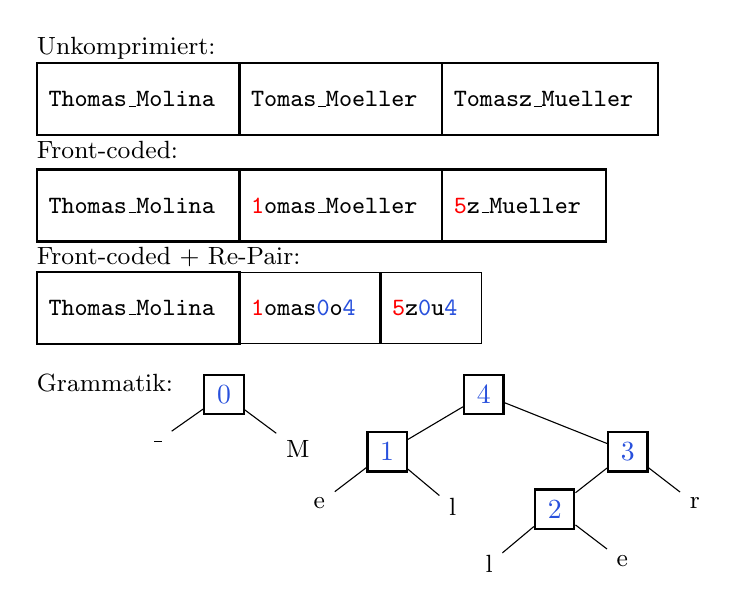
\begin{tikzpicture}
		
		% ------------------- Row 1: Unkomprimiert -------------------
		\node[lab] (labU) at (0,4.6) {Unkomprimiert:};
		
		\matrix (mU) [matrix of nodes,
		nodes={boxcell, tt},
		row sep=0pt, column sep=0pt,
		anchor=west
		] at (0,3.95) {
			\spaced{Thomas\_Molina} &
			\spaced{Tomas\_Moeller} &
			\spaced{Tomasz\_Mueller} \\
		};
		% outer frame (optional stronger outline)
		\draw[frame] (mU-1-1.north west) rectangle (mU-1-3.south east);
		
		% ------------------- Row 2: Front-coded (nicht übersetzen) -------------------
		\node[lab] (labF) at (0,3.3) {Front-coded:};
		
		\matrix (mF) [matrix of nodes,
		nodes={boxcell, tt},
		row sep=0pt, column sep=0pt,
		anchor=west
		] at (0,2.60) {
			\spaced{Thomas\_Molina} &
			\spaced{\red{1}omas\_Moeller} &
			\spaced{\red{5}z\_Mueller} \\
		};
		\draw[frame] (mF-1-1.north west) rectangle (mF-1-3.south east);
		
		% ------------------- Row 3: Front-coded + Re-Pair -------------------
		\node[lab] (labFR) at (0,1.95) {Front-coded + Re-Pair:};
		
		\matrix (mFR) [matrix of nodes,
		nodes={boxcell, font=\ttfamily\small},
		row sep=0pt, column sep=0pt,
		anchor=west
		] at (0,1.3) {
			\spaced{Thomas\_Molina} &
			\spaced{\red{1}omas\blue{0}o\blue{4}} & 
			\spaced{\red{5}z\blue{0}u\blue{4}} \\
		};
		
		\draw[frame] (mFR-1-1.north west) rectangle (mFR-1-1.south east);

		
		% ------------------- Grammar tree (German label) -------------------
		\node[lab] (labG) at (0,0.35) {Grammatik:};
		
		\node[nt] (n0) at (2.5,0.2) {0};
		\node[term] (t_) [below left=2mm and 4mm of n0] {\_};
		\node[term] (tM) [below right=2mm and 4mm of n0] {M};
		\draw (n0) -- (t_);
		\draw (n0) -- (tM);
		
		\node[nt] (n4) at (5.8,0.2) {4};
		\node[nt] (n1) [below left=2mm and 7mm of n4] {1};
		\node[nt] (n3) [below right=2mm and 13mm of n4] {3};
		\draw (n4) -- (n1);
		\draw (n4) -- (n3);
		
		\node[term] (te1) [below left=2mm and 4mm of n1] {e};
		\node[term] (tl1) [below right=2mm and 4mm of n1] {l};
		\draw (n1) -- (te1);
		\draw (n1) -- (tl1);
		
		\node[nt] (n2) [below left=2mm and 4mm of n3] {2};
		\node[term] (tr) [below right=2mm and 4mm of n3] {r};
		\draw (n3) -- (n2);
		\draw (n3) -- (tr);
		
		\node[term] (tl2) [below left=2mm and 4mm of n2] {l};
		\node[term] (te2) [below right=2mm and 4mm of n2] {e};
		\draw (n2) -- (tl2);
		\draw (n2) -- (te2);
		
	\end{tikzpicture}
\end{document}
